% Computer Networks homework template.
% Environment: Windows10 Home + TeXLive2019 + Visual Studio Code.
% Environment: Deepin 15.11 + TeXLive2019 + Visual Studio Code.
\documentclass[a4paper,UTF8]{article}
\usepackage{ctex}
\ctexset{
proofname = \heiti{证明}
}

\usepackage{upgreek}
\usepackage{float}
%代码段设置
\usepackage{listings}
\lstset{breaklines}  %让LaTeX自动将长的代码行换行排版
\lstset{extendedchars=false}   %这一条命令可以解决代码跨页时,章节标题,页眉等汉字不显示的问题
\lstset{
    language=C++, %用于设置语言为C++
    identifierstyle=,
    basicstyle=\ttfamily,
    stringstyle=\ttfamily,
    showstringspaces=false,
    frame=shadowbox, %边框
    captionpos=b
}

\usepackage{amsmath, amssymb, amsthm}
% amsmath: equation*, amssymb: mathbb, amsthm: proof
\usepackage{moreenum}
\usepackage{mathtools}
\usepackage{url}
\usepackage{bm}
\usepackage{enumitem}
\usepackage{graphicx}
\usepackage{subcaption}
\usepackage{booktabs} % toprule
\usepackage[mathcal]{eucal}
\usepackage[thehwcnt = 4]{iidef}

\thecourseinstitute{中国海洋大学}
\thecoursename{计算机网络}
\theterm{2019秋季学期}
\hwname{作业}
\slname{\heiti{解}}
\begin{document}
\courseheader
\name{姓名:秦浩 \qquad 学号:17020031051}

\setlength{\itemsep}{3\parskip}

\section{实验环境} 
\item[1] Deepin 15.11 x64
\item[-] gcc (Debian 6.3.0-18+deb9u1) 6.3.0
\item[-] g++ (Debian 6.3.0-18+deb9u1) 6.3.0
\item[2] Windows 10 x64
\item[-] Visual C++ 6.0

\section{编程作业}
\subsection{编程实现PING功能}
程序代码如下ping.c所示。ping命令的工作原理是:向网络上的另一个主机系统发送ICMP报文,如果指定系统得到了报文,它将把报文一模一样地传回给发送者。\\
\item[2.1.1] IP报头数据结构为:
\begin{lstlisting}
    struct ip
    {
    #if __BYTE_ORDER == __LITTLE_ENDIAN
        unsigned int ip_hl:4;       /* header length */
        unsigned int ip_v:4;        /* version */
    #endif
    #if __BYTE_ORDER == __BIG_ENDIAN
        unsigned int ip_v:4;        /* version */
        unsigned int ip_hl:4;       /* header length */
    #endif
        u_int8_t ip_tos;            /* type of service */
        u_short ip_len;         /* total length */
        u_short ip_id;          /* identification */
        u_short ip_off;         /* fragment offset field */
    #define IP_RF 0x8000            /* reserved fragment flag */
    #define IP_DF 0x4000            /* dont fragment flag */
    #define IP_MF 0x2000            /* more fragments flag */
    #define IP_OFFMASK 0x1fff       /* mask for fragmenting bits */
        u_int8_t ip_ttl;            /* time to live */
        u_int8_t ip_p;          /* protocol */
        u_short ip_sum;         /* checksum */
        struct in_addr ip_src, ip_dst;  /* source and dest address */
    };
\end{lstlisting}
\item[2.1.2] ICMP数据结构为:
\begin{lstlisting}
    struct icmp
    {
    u_int8_t  icmp_type;  /* type of message, see below */
    u_int8_t  icmp_code;  /* type sub code */
    u_int16_t icmp_cksum; /* ones complement checksum of struct */
    union
    {
        u_char ih_pptr;     /* ICMP_PARAMPROB */
        struct in_addr ih_gwaddr;   /* gateway address */
        struct ih_idseq     /* echo datagram */
        {
        u_int16_t icd_id;
        u_int16_t icd_seq;
        } ih_idseq;
        u_int32_t ih_void;
        /* ICMP_UNREACH_NEEDFRAG -- Path MTU Discovery (RFC1191) */
        struct ih_pmtu
        {
        u_int16_t ipm_void;
        u_int16_t ipm_nextmtu;
        } ih_pmtu;
        struct ih_rtradv
        {
        u_int8_t irt_num_addrs;
        u_int8_t irt_wpa;
        u_int16_t irt_lifetime;
        } ih_rtradv;
    } icmp_hun;
    #define icmp_pptr   icmp_hun.ih_pptr
    #define icmp_gwaddr icmp_hun.ih_gwaddr
    #define icmp_id     icmp_hun.ih_idseq.icd_id
    #define icmp_seq        icmp_hun.ih_idseq.icd_seq
    #define icmp_void   icmp_hun.ih_void
    #define icmp_pmvoid icmp_hun.ih_pmtu.ipm_void
    #define icmp_nextmtu    icmp_hun.ih_pmtu.ipm_nextmtu
    #define icmp_num_addrs  icmp_hun.ih_rtradv.irt_num_addrs
    #define icmp_wpa    icmp_hun.ih_rtradv.irt_wpa
    #define icmp_lifetime   icmp_hun.ih_rtradv.irt_lifetime
    union
    {
        struct
        {
        u_int32_t its_otime;
        u_int32_t its_rtime;
        u_int32_t its_ttime;
        } id_ts;
        struct
        {
        struct ip idi_ip;
        /* options and then 64 bits of data */
        } id_ip;
        struct icmp_ra_addr id_radv;
        u_int32_t   id_mask;
        u_int8_t    id_data[1];
    } icmp_dun;
    #define icmp_otime  icmp_dun.id_ts.its_otime
    #define icmp_rtime  icmp_dun.id_ts.its_rtime
    #define icmp_ttime  icmp_dun.id_ts.its_ttime
    #define icmp_ip     icmp_dun.id_ip.idi_ip
    #define icmp_radv   icmp_dun.id_radv
    #define icmp_mask   icmp_dun.id_mask
    #define icmp_data   icmp_dun.id_data
    };
\end{lstlisting}
程序运行结果如图1所示:
\begin{figure}[htbp]
    \centering
    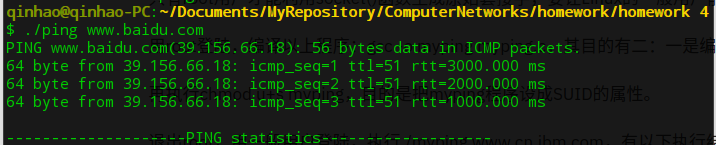
\includegraphics[width=1\textwidth]{ping.png}
    \caption{ping.c运行结果}
    \label{pingImg}
\end{figure}
\subsection{获取所在局域网的子网掩码,用实现的PING程序查询子网内所有IP地址的在线状态}
连接的校园网为OUC-AUTO,本机地址为10.115.240.252,子网掩码为255.255.192.0。
\subsection{编程实现tracert功能}
程序源码如下tacert.cpp所示。程序实现是向目的主机发送一个 ICMP 回显请求报文,初始时 TTL (IP 头部生存时间(time to live)) 等于 1 ,这样当该数据报抵达途中的第一个路由器时,TTL 的值就被减为 0,导致发送超时错误,因此该路由生成一份 ICMP 超时差错报文返回给源主机。随后,主机将数据报的 TTL 值递增 1 ,以便 IP 报能传送到下一个路由器,并由下一个路由器生成 ICMP 超时差错报文返回给源主机。不断重复这个过程,直到数据报达到目的主机或超过跳数限制,到达目的主机后,目的主机返回 ICMP 回显应答报文。这样,源主机只需要对返回的每一份 ICMP 报文进行解析处理,就可以掌握数据报从源主机到达目的主机途中所经过的路由信息。\\
用到的数据结构如下所示:
\begin{lstlisting}
    //IP报头
    typedef struct IP_HEADER
    {
        unsigned char hdr_len:4;       //4位头部长度
        unsigned char version:4;       //4位版本号
        unsigned char tos;             //8位服务类型
        unsigned short total_len;      //16位总长度
        unsigned short identifier;     //16位标识符
        unsigned short frag_and_flags; //3位标志加13位片偏移
        unsigned char ttl;             //8位生存时间
        unsigned char protocol;        //8位上层协议号
        unsigned short checksum;       //16位校验和
        unsigned long sourceIP;        //32位源IP地址
        unsigned long destIP;          //32位目的IP地址
    } IP_HEADER;

    //ICMP报头
    typedef struct ICMP_HEADER
    {
        BYTE type;    //8位类型字段
        BYTE code;    //8位代码字段
        USHORT cksum; //16位校验和
        USHORT id;    //16位标识符
        USHORT seq;   //16位序列号
    } ICMP_HEADER;

    //报文解码结构
    typedef struct DECODE_RESULT
    {
        USHORT usSeqNo;        //序列号
        DWORD dwRoundTripTime; //往返时间
        in_addr dwIPaddr;      //返回报文的IP地址
    }DECODE_RESULT;
\end{lstlisting}
\subsection{用实现的tracert程序查询到jd.com的每一跳路由器IP地址,查询IP名称并分析层级关系,画出一个可能的IP层次关系图}
程序运行结果如图2所示:\\
\begin{figure}[htbp]
    \centering
    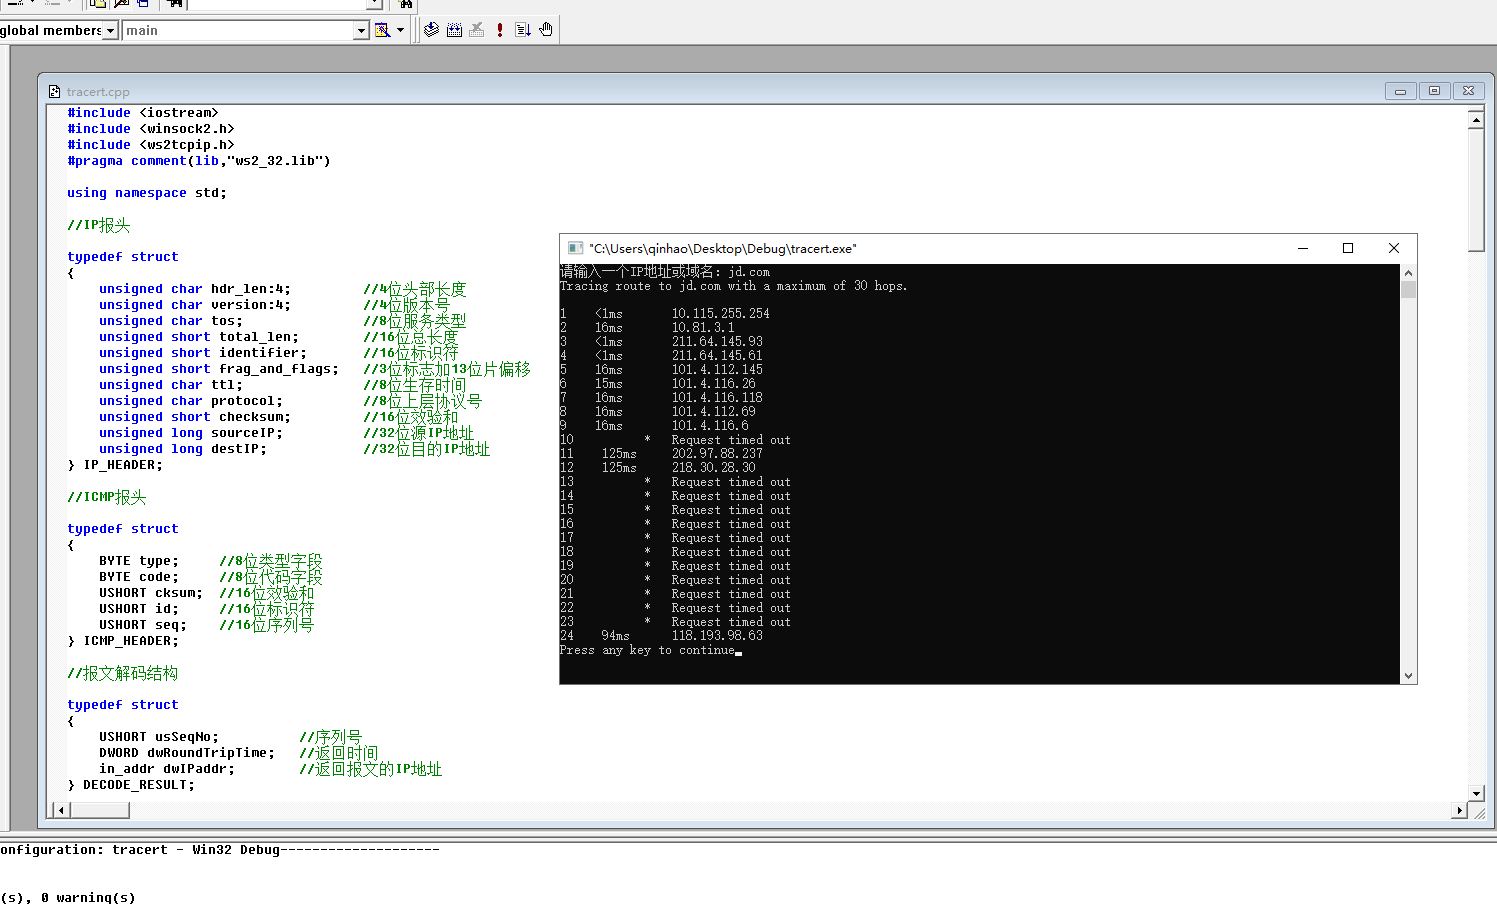
\includegraphics[width=1\textwidth]{tracert}
    \caption{tracert.cpp运行结果}
    \label{tracert}
\end{figure}
IP名称如下图3所示:\\
\begin{figure}[htbp]
    \centering
    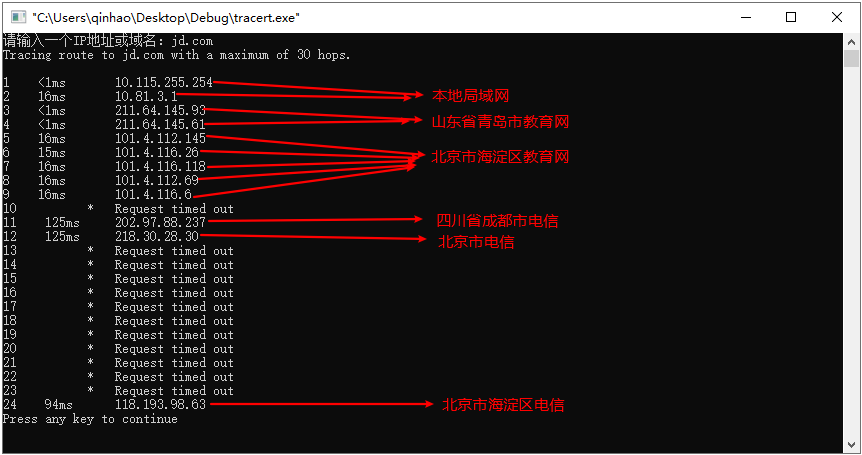
\includegraphics[width=1\textwidth]{tracert_path}
    \caption{tracert.cpp运行结果}
    \label{tracert_path}
\end{figure}
层级关系如下图4所示:\\
\begin{figure}[htbp]
    \centering
    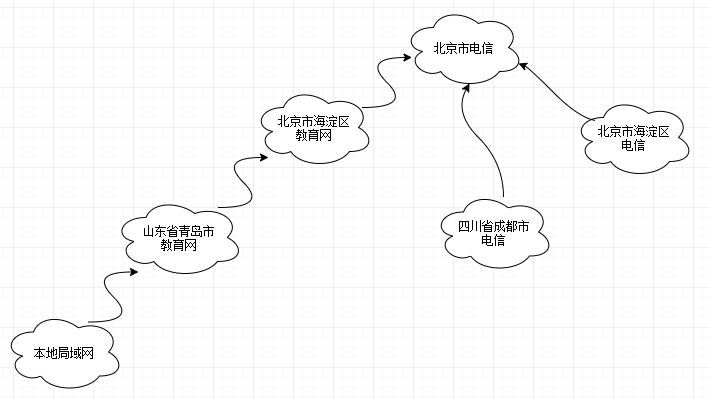
\includegraphics[width=1\textwidth]{tracert_level}
    \caption{可能的层次关系}
    \label{tracert_level}
\end{figure}

\section{程序源码}
\subsection{ping.c}
\begin{lstlisting}

    #include <stdio.h>
    #include <signal.h>
    #include <arpa/inet.h>
    #include <sys/types.h>
    #include <sys/socket.h>
    #include <unistd.h>
    #include <netinet/in.h>
    #include <netinet/ip.h>
    #include <netinet/ip_icmp.h>
    #include <netdb.h>
    #include <setjmp.h>
    #include <errno.h>

    #define PACKET_SIZE 4096
    #define MAX_WAIT_TIME 5
    #define MAX_NO_PACKETS 3

    char sendpacket[PACKET_SIZE];
    char recvpacket[PACKET_SIZE];
    int sockfd, datalen = 56;
    int nsend = 0, nreceived = 0;
    struct sockaddr_in dest_addr;
    pid_t pid;
    struct sockaddr_in from;
    struct timeval tvrecv;

    void statistics(int signo);
    unsigned short cal_chksum(unsigned short *addr, int len);
    int pack(int pack_no);
    void send_packet(void);
    void recv_packet(void);
    int unpack(char *buf, int len);
    void tv_sub(struct timeval *out, struct timeval *in);

    void statistics(int signo)
    {
        printf("\n--------------------PING statistics-------------------\n");
        printf("%d packets transmitted, %d received , %%%d lost\n", nsend, nreceived,
            (nsend - nreceived) / nsend * 100);
        close(sockfd);
        exit(1);
    }
    /*校验和算法*/
    unsigned short cal_chksum(unsigned short *addr, int len)
    {
        int nleft = len;
        int sum = 0;
        unsigned short *w = addr;
        unsigned short answer = 0;

        /*把ICMP报头二进制数据以2字节为单位累加起来*/
        while (nleft > 1)
        {
            sum += *w++;
            nleft -= 2;
        }
        /*若ICMP报头为奇数个字节,会剩下最后一字节。把最后一个字节视为一个2字节数据的高字节,这个2字节数据的低字节为0,继续累加*/
        if (nleft == 1)
        {
            *(unsigned char *)(&answer) = *(unsigned char *)w;
            sum += answer;
        }
        sum = (sum >> 16) + (sum & 0xffff);
        sum += (sum >> 16);
        answer = ~sum;
        return answer;
    }
    /*设置ICMP报头*/
    int pack(int pack_no)
    {
        int i, packsize;
        struct icmp *icmp;
        struct timeval *tval;
        icmp = (struct icmp *)sendpacket;
        icmp->icmp_type = ICMP_ECHO;
        icmp->icmp_code = 0;
        icmp->icmp_cksum = 0;
        icmp->icmp_seq = pack_no;
        icmp->icmp_id = pid;
        packsize = 8 + datalen;
        tval = (struct timeval *)icmp->icmp_data;
        gettimeofday(tval, NULL);                                        /*记录发送时间*/
        icmp->icmp_cksum = cal_chksum((unsigned short *)icmp, packsize); /*校验算法*/
        return packsize;
    }
    /*发送三个ICMP报文*/
    void send_packet()
    {
        int packetsize;
        while (nsend < MAX_NO_PACKETS)
        {
            nsend++;
            packetsize = pack(nsend); /*设置ICMP报头*/
            if (sendto(sockfd, sendpacket, packetsize, 0,
                    (struct sockaddr *)&dest_addr, sizeof(dest_addr)) < 0)
            {
                perror("sendto error");
                continue;
            }
            sleep(1); /*每隔一秒发送一个ICMP报文*/
        }
    }
    /*接收所有ICMP报文*/
    void recv_packet()
    {
        int n, fromlen;
        extern int errno;
        signal(SIGALRM, statistics);
        fromlen = sizeof(from);
        while (nreceived < nsend)
        {
            alarm(MAX_WAIT_TIME);
            if ((n = recvfrom(sockfd, recvpacket, sizeof(recvpacket), 0,
                            (struct sockaddr *)&from, &fromlen)) < 0)
            {
                if (errno == EINTR)
                    continue;
                perror("recvfrom error");
                continue;
            }
            gettimeofday(&tvrecv, NULL); /*记录接收时间*/
            if (unpack(recvpacket, n) == -1)
                continue;
            nreceived++;
        }
    }
    /*剥去ICMP报头*/
    int unpack(char *buf, int len)
    {
        int i, iphdrlen;
        struct ip *ip;
        struct icmp *icmp;
        struct timeval *tvsend;
        double rtt;
        ip = (struct ip *)buf;
        iphdrlen = ip->ip_hl << 2;              /*求ip报头长度,即ip报头的长度标志乘4*/
        icmp = (struct icmp *)(buf + iphdrlen); /*越过ip报头,指向ICMP报头*/
        len -= iphdrlen;                        /*ICMP报头及ICMP数据报的总长度*/
        if (len < 8)                            /*小于ICMP报头长度则不合理*/
        {
            printf("ICMP packets\'s length is less than 8\n");
            return -1;
        }
        /*确保所接收的是我所发的的ICMP的回应*/
        if ((icmp->icmp_type == ICMP_ECHOREPLY) && (icmp->icmp_id == pid))
        {
            tvsend = (struct timeval *)icmp->icmp_data;
            tv_sub(&tvrecv, tvsend);                            /*接收和发送的时间差*/
            rtt = tvrecv.tv_sec * 1000 + tvrecv.tv_usec / 1000; /*以毫秒为单位计算rtt*/
            /*显示相关信息*/
            printf("%d byte from %s: icmp_seq=%u ttl=%d rtt=%.3f ms\n",
                len,
                inet_ntoa(from.sin_addr),
                icmp->icmp_seq,
                ip->ip_ttl,
                rtt);
        }
        else
            return -1;
    }
    int main(int argc, char *argv[])
    {
        struct hostent *host;
        struct protoent *protocol;
        unsigned long inaddr = 0l;
        int waittime = MAX_WAIT_TIME;
        int size = 50 * 1024;
        if (argc < 2)
        {
            printf("usage:%s hostname/IP address\n", argv[0]);
            exit(1);
        }
        if ((protocol = getprotobyname("icmp")) == NULL)
        {
            perror("getprotobyname");
            exit(1);
        }
        /*生成使用ICMP的原始套接字,这种套接字只有root才能生成*/
        if ((sockfd = socket(AF_INET, SOCK_RAW, protocol->p_proto)) < 0)
        {
            perror("socket error");
            exit(1);
        }
        /* 回收root权限,设置当前用户权限*/
        setuid(getuid());
        /*扩大套接字接收缓冲区到50K这样做主要为了减小接收缓冲区溢出的
            的可能性,若无意中ping一个广播地址或多播地址,将会引来大量应答*/
        setsockopt(sockfd, SOL_SOCKET, SO_RCVBUF, &size, sizeof(size));
        bzero(&dest_addr, sizeof(dest_addr));
        dest_addr.sin_family = AF_INET;
        /*判断是主机名还是ip地址*/
        if (inaddr = inet_addr(argv[1]) == INADDR_NONE)
        {
            if ((host = gethostbyname(argv[1])) == NULL) /*是主机名*/
            {
                perror("gethostbyname error");
                exit(1);
            }
            memcpy((char *)&dest_addr.sin_addr, host->h_addr, host->h_length);
        }
        else /*是ip地址*/
            memcpy((char *)&dest_addr, (char *)&inaddr, host->h_length);
        /*获取main的进程id,用于设置ICMP的标志符*/
        pid = getpid();
        printf("PING %s(%s): %d bytes data in ICMP packets.\n", argv[1],
            inet_ntoa(dest_addr.sin_addr), datalen);
        send_packet();       /*发送所有ICMP报文*/
        recv_packet();       /*接收所有ICMP报文*/
        statistics(SIGALRM); /*进行统计*/
        return 0;
    }
    /*两个timeval结构相减*/
    void tv_sub(struct timeval *out, struct timeval *in)
    {
        if ((out->tv_usec -= in->tv_usec) < 0)
        {
            --out->tv_sec;
            out->tv_usec += 1000000;
        }
        out->tv_sec -= in->tv_sec;
    }

\end{lstlisting}
\subsection{tracert.cpp}
\begin{lstlisting}
    #include <iostream>
    #include <winsock2.h>       
    #include <ws2tcpip.h>
    using namespace std;

    #pragma comment(lib, "Ws2_32.lib")

    //IP报头
    typedef struct IP_HEADER
    {
        unsigned char hdr_len:4;       //4位头部长度
        unsigned char version:4;       //4位版本号
        unsigned char tos;             //8位服务类型
        unsigned short total_len;      //16位总长度
        unsigned short identifier;     //16位标识符
        unsigned short frag_and_flags; //3位标志加13位片偏移
        unsigned char ttl;             //8位生存时间
        unsigned char protocol;        //8位上层协议号
        unsigned short checksum;       //16位校验和
        unsigned long sourceIP;        //32位源IP地址
        unsigned long destIP;          //32位目的IP地址
    } IP_HEADER;

    //ICMP报头
    typedef struct ICMP_HEADER
    {
        BYTE type;    //8位类型字段
        BYTE code;    //8位代码字段
        USHORT cksum; //16位校验和
        USHORT id;    //16位标识符
        USHORT seq;   //16位序列号
    } ICMP_HEADER;

    //报文解码结构
    typedef struct DECODE_RESULT
    {
        USHORT usSeqNo;        //序列号
        DWORD dwRoundTripTime; //往返时间
        in_addr dwIPaddr;      //返回报文的IP地址
    }DECODE_RESULT;

    //计算网际校验和函数
    USHORT checksum( USHORT *pBuf, int iSize )
    {
        unsigned long cksum = 0;
        while( iSize > 1 )
        {
            cksum += *pBuf++;
            iSize -= sizeof(USHORT);
        }
        if( iSize )//如果 iSize 为正,即为奇数个字节
        {
            cksum += *(UCHAR *)pBuf; //则在末尾补上一个字节,使之有偶数个字节
        }
        cksum  = ( cksum >> 16 ) + ( cksum&0xffff );
        cksum += ( cksum >> 16 );
        return (USHORT)( ~cksum );
    }

    //对数据包进行解码
    BOOL DecodeIcmpResponse(char * pBuf, int iPacketSize, DECODE_RESULT &DecodeResult,
                            BYTE ICMP_ECHO_REPLY, BYTE  ICMP_TIMEOUT)
    {
        //检查数据报大小的合法性
        IP_HEADER* pIpHdr = ( IP_HEADER* )pBuf;
        int iIpHdrLen = pIpHdr->hdr_len * 4;    //ip报头的长度是以4字节为单位的

        //若数据包大小 小于 IP报头 + ICMP报头,则数据报大小不合法
        if ( iPacketSize < ( int )( iIpHdrLen + sizeof( ICMP_HEADER ) ) )
            return FALSE;

        //根据ICMP报文类型提取ID字段和序列号字段
        ICMP_HEADER *pIcmpHdr = ( ICMP_HEADER * )( pBuf + iIpHdrLen );//ICMP报头 = 接收到的缓冲数据 + IP报头
        USHORT usID, usSquNo;

        if( pIcmpHdr->type == ICMP_ECHO_REPLY )    //ICMP回显应答报文
        {
            usID = pIcmpHdr->id;        //报文ID
            usSquNo = pIcmpHdr->seq;    //报文序列号
        }
        else if( pIcmpHdr->type == ICMP_TIMEOUT )//ICMP超时差错报文
        {
            char * pInnerIpHdr = pBuf + iIpHdrLen + sizeof( ICMP_HEADER ); //载荷中的IP头
            int iInnerIPHdrLen = ( ( IP_HEADER * )pInnerIpHdr )->hdr_len * 4; //载荷中的IP头长
            ICMP_HEADER * pInnerIcmpHdr = ( ICMP_HEADER * )( pInnerIpHdr + iInnerIPHdrLen );//载荷中的ICMP头

            usID = pInnerIcmpHdr->id;        //报文ID
            usSquNo = pInnerIcmpHdr->seq;    //序列号
        }
        else
        {
            return false;
        }

        //检查ID和序列号以确定收到期待数据报
        if( usID != ( USHORT )GetCurrentProcessId() || usSquNo != DecodeResult.usSeqNo )
        {
            return false;
        }
        //记录IP地址并计算往返时间
        DecodeResult.dwIPaddr.s_addr = pIpHdr->sourceIP;
        DecodeResult.dwRoundTripTime = GetTickCount() - DecodeResult.dwRoundTripTime;

        //处理正确收到的ICMP数据报
        if ( pIcmpHdr->type == ICMP_ECHO_REPLY || pIcmpHdr->type == ICMP_TIMEOUT )
        {
            //输出往返时间信息
            if(DecodeResult.dwRoundTripTime)
                cout<<"      "<<DecodeResult.dwRoundTripTime<<"ms"<<flush;
            else
                cout<<"      "<<"<1ms"<<flush;
        }
        return true;
    }

    void main()
    {
        //初始化Windows sockets网络环境
        WSADATA wsa;
        WSAStartup( MAKEWORD(2,2), &wsa );
        char IpAddress[255];
        cout<<"请输入一个IP地址或域名:";
        cin>>IpAddress;

        //得到IP地址
        u_long ulDestIP = inet_addr( IpAddress );

        //转换不成功时按域名解析
        if( ulDestIP == INADDR_NONE )
        {
            hostent * pHostent = gethostbyname( IpAddress );
            if( pHostent )
            {
                ulDestIP = ( *( in_addr* )pHostent->h_addr).s_addr;
            }
            else
            {
                cout<<"输入的IP地址或域名无效!"<<endl;
                WSACleanup();
                return;
            }
        }
        cout<<"Tracing roote to "<<IpAddress<<" with a maximum of 30 hops.\n"<<endl;

        //填充目的端socket地址
        sockaddr_in destSockAddr;
        ZeroMemory( &destSockAddr, sizeof( sockaddr_in ) );
        destSockAddr.sin_family = AF_INET;
        destSockAddr.sin_addr.s_addr = ulDestIP;

        //创建原始套接字
        SOCKET sockRaw = WSASocket( AF_INET, SOCK_RAW, IPPROTO_ICMP, NULL, 0, WSA_FLAG_OVERLAPPED );

        //超时时间
        int iTimeout = 3000;

        //设置接收超时时间
        setsockopt( sockRaw, SOL_SOCKET, SO_RCVTIMEO, (char *)&iTimeout, sizeof( iTimeout ) );

        //设置发送超时时间
        setsockopt(sockRaw,SOL_SOCKET,SO_SNDTIMEO,(char *)&iTimeout,sizeof(iTimeout));

        //构造ICMP回显请求消息,并以TTL递增的顺序发送报文
        //ICMP类型字段
        const BYTE ICMP_ECHO_REQUEST = 8;    //请求回显
        const BYTE ICMP_ECHO_REPLY   = 0;    //回显应答
        const BYTE ICMP_TIMEOUT      = 11;   //传输超时

        //其他常量定义
        const int DEF_ICMP_DATA_SIZE   = 32;    //ICMP报文默认数据字段长度
        const int MAX_ICMP_PACKET_SIZE = 1024;  //ICMP报文最大长度(包括报头)
        const DWORD DEF_ICMP_TIMEOUT   = 3000;  //回显应答超时时间
        const int DEF_MAX_HOP          = 30;    //最大跳站数

        //填充ICMP报文中每次发送时不变的字段
        char IcmpSendBuf[ sizeof( ICMP_HEADER ) + DEF_ICMP_DATA_SIZE ];//发送缓冲区
        memset( IcmpSendBuf, 0, sizeof( IcmpSendBuf ) );               //初始化发送缓冲区
        char IcmpRecvBuf[ MAX_ICMP_PACKET_SIZE ];                      //接收缓冲区
        memset( IcmpRecvBuf, 0, sizeof( IcmpRecvBuf ) );               //初始化接收缓冲区

        ICMP_HEADER * pIcmpHeader = ( ICMP_HEADER* )IcmpSendBuf;
        pIcmpHeader->type = ICMP_ECHO_REQUEST; //类型为请求回显
        pIcmpHeader->code = 0;                //代码字段为0
        pIcmpHeader->id   = (USHORT)GetCurrentProcessId();    //ID字段为当前进程号
        memset( IcmpSendBuf + sizeof( ICMP_HEADER ), 'E', DEF_ICMP_DATA_SIZE );//数据字段

        USHORT usSeqNo      = 0;            //ICMP报文序列号
        int iTTL            = 1;            //TTL初始值为1
        BOOL bReachDestHost = FALSE;        //循环退出标志
        int iMaxHot         = DEF_MAX_HOP;  //循环的最大次数
        DECODE_RESULT DecodeResult;    //传递给报文解码函数的结构化参数
        while( !bReachDestHost && iMaxHot-- )
        {
            //设置IP报头的TTL字段
            setsockopt( sockRaw, IPPROTO_IP, IP_TTL, (char *)&iTTL, sizeof(iTTL) );
            cout<<iTTL<<flush;    //输出当前序号,flush表示将缓冲区的内容马上送进cout,把输出缓冲区刷新

            //填充ICMP报文中每次发送变化的字段
            ((ICMP_HEADER *)IcmpSendBuf)->cksum = 0;                   //校验和先置为0
            ((ICMP_HEADER *)IcmpSendBuf)->seq   = htons(usSeqNo++);    //填充序列号
            ((ICMP_HEADER *)IcmpSendBuf)->cksum = 
                checksum( ( USHORT * )IcmpSendBuf, sizeof( ICMP_HEADER ) + DEF_ICMP_DATA_SIZE ); //计算校验和

            //记录序列号和当前时间
            DecodeResult.usSeqNo         = ( ( ICMP_HEADER* )IcmpSendBuf )->seq;    //当前序号
            DecodeResult.dwRoundTripTime = GetTickCount();                          //当前时间

            //发送TCP回显请求信息
            sendto( sockRaw, IcmpSendBuf, sizeof(IcmpSendBuf), 0, (sockaddr*)&destSockAddr, sizeof(destSockAddr) );

            //接收ICMP差错报文并进行解析处理
            sockaddr_in from;           //对端socket地址
            int iFromLen = sizeof(from);//地址结构大小
            int iReadDataLen;           //接收数据长度
            while(1)
            {
                //接收数据
                iReadDataLen = recvfrom( sockRaw, IcmpRecvBuf, MAX_ICMP_PACKET_SIZE, 0, (sockaddr*)&from, &iFromLen );
                if( iReadDataLen != SOCKET_ERROR )//有数据到达
                {
                    //对数据包进行解码
                    if(DecodeIcmpResponse( IcmpRecvBuf, iReadDataLen, DecodeResult, ICMP_ECHO_REPLY, ICMP_TIMEOUT ) )
                    {
                        //到达目的地,退出循环
                        if( DecodeResult.dwIPaddr.s_addr == destSockAddr.sin_addr.s_addr )
                            bReachDestHost = true;
                        //输出IP地址
                        cout<<'\t'<<inet_ntoa( DecodeResult.dwIPaddr )<<endl;
                        break;
                    }
                }
                else if( WSAGetLastError() == WSAETIMEDOUT )    //接收超时,输出*号
                {
                    cout<<"         *"<<'\t'<<"Request timed out."<<endl;
                    break;
                }
                else
                {
                    break;
                }
            }
            iTTL++;    //递增TTL值
        }
    }
\end{lstlisting}
\end{document}
\begin{equation}
\end{equation}